\chapter{Tecnologias}

\section{\textit{Framework}}
Segundo \citeonline{artigo_oo_reuso_software}, a programação orientada a objetos é muita vezes utilizada para promover o reuso de software. Para \citeonline{artigo_reuso_classes}, algumas linguagens, como \textit{Smalltalk}, são utilizadas tanto para reduzir o tempo de desenvolvimento quanto o custo de manutenções, simplificando a criação de novos sistemas e de novas versões para sistemas já existentes, afirma, também, que “componentes de um programa devem ser projetados para reusabilidade”, o qual pode ser visto de maneira clara, por exemplo, em um sistema bancário, pela sua necessidade de recebimento e troca de informações com diversos outros sistemas.

Novamente, segundo \citeonline{artigo_reuso_classes}, um “design abstrato orientado a objetos”, também chamado de \textit{framework}, consiste em uma classe abstrata para cada principal componente, onde as interfaces entre os componentes do design são definidas em termos de um conjunto de mensagens, além disso, “\textit{frameworks} proveem uma maneira de reutilizar código que é resistente a mais tentativas de reusos convencionais”, ou seja, componentes independentes de uma aplicação podem ser reutilizados mais facilmente.

\citeonline{artigo_reuso_classes}, compara “programas esqueletos” com \textit{frameworks}, os quais consistem em uma abordagem tradicional de reutilização de código e na garantia de consistência entre todos os componentes de um sistema sobre a mudança de algum requisito, respectivamente. O autor também realiza uma comparação entre os \textit{frameworks} do tipo “caixa-branca” e “caixa-preta”, onde o primeiro é responsável por especificar o comportamento de uma aplicação adicionando-se métodos para subclasses de uma ou mais de suas classes, ou seja, a implementação deste tipo de \textit{framework} deve ser conhecida para sua utilização, já o segundo consiste no uso de um protocolo responsável por definir uma interface entre os componentes, assim, o usuário precisaria entender apenas como funciona a interface externa dos componentes para utilizá-los.

\section{\textit{Django}}
O \textit{Django} é um \textit{framework} para desenvolvimento \textit{web}. A linguagem de programação usada com esse \textit{framework} é o Python.

O Python é uma linguagem de programação de alto nível, interpretada, imperativa, orientada a objetos, de tipagem dinâmica e forte. Foi lançada por Guido van Rossum em 1991.

A arquitetura utilizada no \textit{Django} basea-se no MTV (Model-Template-View), a qual diferencia-se um pouco do tradicional MVC (Model, View, Controller), arquitetura na qual separam-se as regras de negócios (Controller), os dados e métodos de acessos aos mesmos (Model) e as regras de apresentação (View).

No caso da arquitetura MTV, o framework \textit{Django} é o que faz as vezes de controlador da arquitetura MVC. Sendo assim, na arquitetura MTV, o Controller não é responsável pela lógica do negócio e sim pelo funcionamento do sistema. Além de models, views e templates, no \textit{Django} há também o URL dispatcher, middlewares e handlers e são estes que são encarados como Controller.

O URL dispatcher é o componente responsável em analisar os endereços requisitados pelo cliente e redirecionar essa requisição para a aplicação correta. Já o middleware é um conjunto de componentes que realizam pré e pós filtragens nas requisições, o que possibilita funcionalidade como internacionalização de uma aplicação e gerenciamento de sessões autenticadas.

No Model, são escritas as classes que designarão as tabelas no banco de dados. A manipulação dessas tabelas ocorre através do ORM (mapeamento objeto relacional) e, por isso, não é necessária a escrita de querys em SQL para a persistência dos dados.

A camada View consiste em uma função callback para uma respectiva URL descrevendo qual informação será fornecida. Pensando em separar as informações de suas apresentações foi criado a camada de Template, a qual descreve como as informações serão apresentadas para o usuário.

Com o uso do framework \textit{Django}, um projeto é um conjunto de aplicações. Uma aplicação é uma determinada funcionalidade que compõe um projeto. Por causa disso, há a idéia de aplicações plugáveis no \textit{Django} que é uma aplicação que pode ser usada em mais de um projeto com nenhuma ou quase nenhuma alteração de código. Isso quer dizer que a aplicação deve ter seus próprios modelos, suas próprias views, seus próprios templates e encapsular o máximo possível de código que não se enquadre em um desses elementos.

A Figura \ref{django-arq} ilustra a arquitetura do \textit{Django}:

\begin{figure}[h]
    \centering
    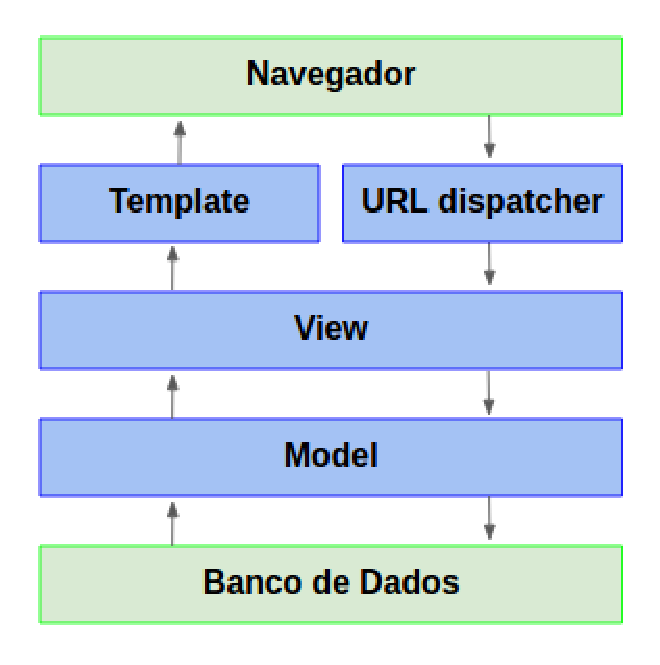
\includegraphics[keepaspectratio=true,scale=0.5]{figuras/django-arquitetura.eps}
    \caption{Arquitetura MTV \textit{Django}}
    \label{django-arq}
\end{figure}

\section{Ferramentas Utilizadas}
    \subsection{\textit{Coverage}}
    Responsável por medir a cobertura de código utilizando ferramentas de análise e rastreando quais
    linhas de teste foram/devem ser executas.

    \subsection{\textit{GitLab CI}}
    Ferramenta que oferece serviço de integração contínua ao projeto.

    \subsection{\textit{Matplotlib}}
    Matplotlib se esforça para produzir qualidade de publicação gráfica 2D para a representação gráfica interativa, publicações científicas, desenvolvimento de interface de usuário e servidores de aplicativos web para múltiplas interfaces de usuário.

    \subsection{\textit{Sphinx}}
    Ferramenta para criação inteligente e estilizada de documentação de códigos em \textit{python} e C/C++. Utiliza \textit{reStructuredText} como sua linguagem de marcação e converte toda a documentação
    para formato html, pdf, epub ou man.

